\documentclass[@BEAMER_OPTIONS@]{beamer}
    @USE_PGFPAGES@

    \usetheme[alternativetitlepage=true,titleline=true]{Torino}
    \setbeamertemplate{navigation symbols}{}
    \setbeamertemplate{note page}[plain]
    \setbeamertemplate{caption}{\insertcaption}

    \usepackage[utf8]{inputenc}
    \usepackage{graphicx}
    \usepackage{subfigure}
    \usepackage{xspace}
    \usepackage{adjustbox}
    \usepackage{tikz}
    \usepackage{relsize}
    \usepackage{fancyvrb}
    \fvset{fontsize=\footnotesize}
    \RecustomVerbatimEnvironment{verbatim}{Verbatim}{}
    \usepgflibrary{arrows}
    \usetikzlibrary{shadows,decorations.pathreplacing,patterns,shapes}
    \tikzstyle{every picture}=[semithick,>=stealth,remember picture]
    \usepackage{inconsolata}
    \usepackage{listings}
    \lstset{
        language=C++,
        basicstyle=\footnotesize\ttfamily,
        keywordstyle=\color{black}\bfseries,
        commentstyle=\color{chameleon1}\it\rmfamily,
        stringstyle=\color{chameleon1},
        numbers=left,
        numberstyle=\tiny,
        aboveskip=-0.02\baselineskip,
        belowskip=-0.02\baselineskip,
        columns=flexible,
        extendedchars=false,
        showstringspaces=false,
        morekeywords={global,kernel,ulong,size_t,get_global_id,get_global_size}
        }
    \newcommand{\code}[1]{\lstinline|#1|}
    \protected\def\plusplus{{\nolinebreak[4]\hspace{-.05em}\raisebox{.4ex}{\relsize{-3}\bf ++}}\xspace}
    \newcommand{\CXX}{{\rm C}\plusplus}
    \newcommand{\CC}{{\rm C99}\xspace}

    \usepackage{ifthen}
\usetikzlibrary{shadows.blur}
\newlength{\ribbonoffset}
\setlength{\ribbonoffset}{3em}

% corner, color, text
\newcommand{\ribbon}[3]{
  \ifthenelse{\equal{#1}{east}}{%
    \tikzset{ribbonrot/.style={rotate=-45}}
  }{%
    \tikzset{ribbonrot/.style={rotate=45}}
  }
  \begin{tikzpicture}[remember picture, overlay]
    \node[ribbonrot, shift={(0, -\ribbonoffset)}] at (current page.north #1) {
      \begin{tikzpicture}[remember picture, overlay,scale=0.5]
        \node[
            fill=#2,
            text centered,
            minimum width=50em,
            minimum height=1.2em,
            blur shadow,
            shadow yshift=0pt,
            shadow xshift=0pt,
            shadow blur radius=.2em,
            shadow opacity=50,
            text=white
            ](fmogh) at (0pt, 0pt) {%
            \fontfamily{phv}\selectfont\bfseries\tiny#3};
        \draw[
            white,
            dashed,
            line width=.04em,
            dash pattern=on .2em off 1.5\pgflinewidth
            ] (-25em,1em) rectangle (25em,-1em);
      \end{tikzpicture}
    };
  \end{tikzpicture}
}

    \newcommand{\forkme}{\ribbon{east}{chameleon1}{\href{https://github.com/ddemidov/vexcl}{Fork me on GitHub}}}
    \newcommand{\singledevice}{\ribbon{east}{chameleon3}{Single device only}}
    \newcommand{\additive}{\ribbon{east}{chameleon3}{Additive expressions}}

    \tikzset{
        treenode/.style={
            draw,
            fill=white,
            blur shadow,
            shadow xshift=1pt,
            shadow yshift=-1pt,
            shadow blur radius=2pt,
            shadow opacity=40
            }
        }


    \title{VexCL}
    \subtitle{Experiences in developing a C++ wrapper library for OpenCL}

    \author{Denis Demidov}
    \institute{
        Kazan Federal University /\\
        Institute of System Research, Russian Academy of Sciences
        \\ \vspace{\baselineskip}
        }
    \date{06.2016, Lausanne}

\begin{document}

%----------------------------------------------------------------------------
\begin{frame}{}
    \titlepage
\end{frame}

\note{ }

%----------------------------------------------------------------------------
\section{Motivation}

%----------------------------------------------------------------------------
\begin{frame}{VexCL~--- a vector expression template library for OpenCL/CUDA}
    \forkme

    \begin{itemize}
        \item Created for ease of \CXX based GPGPU development:
            \begin{itemize}
                \item Convenient notation for vector expressions
                \item OpenCL/CUDA JIT code generation
                \item Easily combined with existing libraries/code
                \item Header-only
            \end{itemize}
            \vspace{\baselineskip}
        \item Supported backends:
            \begin{itemize}
                \item OpenCL (Khronos \CXX bindings, Boost.Compute)
                \item NVIDIA CUDA
            \end{itemize}
            \vspace{\baselineskip}
        \item The source code is available under MIT license:
            \begin{itemize}
                \item \href{https://github.com/ddemidov/vexcl}{https://github.com/ddemidov/vexcl}
            \end{itemize}
            \vspace{\baselineskip}
    \end{itemize}
\end{frame}

\note[itemize]{
\item VexCL is a vector expression template library for OpenCL. It allows you
    to use convenient matlab-like notation for vector operations and it
    generates the appropriate compute kernels for you automatically.
\item The library is header-only, so you don't have to build it to use it. The
    source code of the library is available on GitHub under very liberal
    MIT license.
}

%----------------------------------------------------------------------------
\begin{frame}[fragile]{Motivation/Hello World}
    \setbeamercovered{transparent=40}
    \vspace{-1\baselineskip}
    \begin{columns}
        \begin{column}[t]{0.2\textwidth}
            \begin{exampleblock}{OpenCL}
                \begin{adjustbox}{width=0.19\textwidth, height=\textheight, keepaspectratio}
                    \begin{minipage}{\textwidth}
                        \begin{uncoverenv}<1>
                            \lstinputlisting[linerange={1-8}]{code/hello-opencl.cpp}
                        \end{uncoverenv}
                        \begin{uncoverenv}<1,2>
                            \lstinputlisting[firstnumber=last, linerange={9-35}]{code/hello-opencl.cpp}
                        \end{uncoverenv}
                        \begin{uncoverenv}<1,3>
                            \lstinputlisting[firstnumber=last, linerange={36-48}]{code/hello-opencl.cpp}
                        \end{uncoverenv}
                        \begin{uncoverenv}<1,4>
                            \lstinputlisting[firstnumber=last, linerange={49-86}]{code/hello-opencl.cpp}
                        \end{uncoverenv}
                        \begin{uncoverenv}<1,5>
                            \lstinputlisting[firstnumber=last, linerange={87-90}]{code/hello-opencl.cpp}
                        \end{uncoverenv}
                        \begin{uncoverenv}<1>
                            \lstinputlisting[firstnumber=last, linerange={91}]{code/hello-opencl.cpp}
                        \end{uncoverenv}
                    \end{minipage}
                \end{adjustbox}
            \end{exampleblock}
        \end{column}
        \begin{column}[t]{0.7\textwidth}
            \begin{onlyenv}<1->
            \begin{exampleblock}{VexCL}
                \begin{adjustbox}{width=0.83\textwidth, height=\textheight, keepaspectratio}
                    \begin{minipage}{\textwidth}
                        \begin{uncoverenv}<1>
                            \lstinputlisting[linerange={1-5}]{code/hello-vexcl.cpp}
                        \end{uncoverenv}
                        \begin{uncoverenv}<1,2>
                            \lstinputlisting[firstnumber=last, linerange={6-8}]{code/hello-vexcl.cpp}
                        \end{uncoverenv}
                        \begin{uncoverenv}<1,3>
                            \lstinputlisting[firstnumber=last, linerange={9-13}]{code/hello-vexcl.cpp}
                        \end{uncoverenv}
                        \begin{uncoverenv}<1,4>
                            \lstinputlisting[firstnumber=last, linerange={14-16}]{code/hello-vexcl.cpp}
                        \end{uncoverenv}
                        \begin{uncoverenv}<1,5>
                            \lstinputlisting[firstnumber=last, linerange={17-20}]{code/hello-vexcl.cpp}
                        \end{uncoverenv}
                        \begin{uncoverenv}<1>
                            \lstinputlisting[firstnumber=last, linerange={21}]{code/hello-vexcl.cpp}
                        \end{uncoverenv}
                    \end{minipage}
                \end{adjustbox}
            \end{exampleblock}
            \end{onlyenv}
        \end{column}
    \end{columns}
\end{frame}

\note[itemize]{
\item Here is the simplest example of using vexcl: addition of two vectors on a
    gpu card.
\item The first line is the context initialization. We provide a device filter
    to the context constructor and get all compute devices that satisfy the
    filter. Here we filter by type and get all available GPUs.
\item Data allocation and transfer is also simplified. \code{vex::vector}
    constructor allocates memory on device and possibly transfers initial data
    as well. The parameters here are list of command queues and either size or
    input host vector.
\item Line ten does what's needs to be done here. This simple expression leads
    to automatic kernel generation and launch. And then we copy the results
    back to host and see what we got.
}

%----------------------------------------------------------------------------
\begin{frame}[fragile]{OpenCL/CUDA code is generated from user expressions}
    \begin{columns}
        \begin{column}{0.38\textwidth}
            \begin{exampleblock}{Expression:}
                \begin{lstlisting}
x = 2 * y - sin(z);
                \end{lstlisting}
            \end{exampleblock}
        \end{column}
        \begin{column}{0.55\textwidth}
            \begin{exampleblock}{when compiled with:}
                \begin{onlyenv}<1>
                    \begin{lstlisting}[language=bash,numbers=none]
g++ -DVEXCL_BACKEND_OPENCL -lOpenCL ...
                    \end{lstlisting}
                \end{onlyenv}
                \begin{onlyenv}<2|handout:0>
                    \begin{lstlisting}[language=bash,numbers=none]
g++ -DVEXCL_BACKEND_CUDA -lcuda ...
                    \end{lstlisting}
                \end{onlyenv}
            \end{exampleblock}
        \end{column}
    \end{columns}
    \begin{exampleblock}{Generated kernel:}
        \begin{onlyenv}<1>
            \begin{lstlisting}
kernel void vexcl_vector_kernel
(
  ulong n,
  global double * prm_1,        // x
  int prm_2,                    // 2
  global double * prm_3,        // y
  global double * prm_4         // z
)
{
  for(ulong idx = get_global_id(0); idx < n; idx += get_global_size(0))
  {
    prm_1[idx] = ( ( prm_2 * prm_3[idx] ) - sin( prm_4[idx] ) );
  }
}
            \end{lstlisting}
        \end{onlyenv}
        \begin{onlyenv}<2|handout:0>
            \begin{lstlisting}
extern "C" __global__ void vexcl_vector_kernel (
  ulong n,
  double * prm_1,               // x
  int prm_2,                    // 2
  double * prm_3,               // y
  double * prm_4                // z
)
{
  for(ulong idx = blockDim.x*blockIdx.x + threadIdx.x, grid_size = blockDim.x*gridDim.x;
      idx < n; idx += grid_size)
  {
    prm_1[idx] = ( ( prm_2 * prm_3[idx] ) - sin( prm_4[idx] ) );
  }
}
            \end{lstlisting}
        \end{onlyenv}
    \end{exampleblock}
\end{frame}

\note{ }

%----------------------------------------------------------------------------
\begin{frame}[fragile]{Monte Carlo $\pi$}
    \vspace{-1\baselineskip}
    \begin{columns}
        \begin{column}{0.55\textwidth}
            \begin{itemize}
                \item Compute approximate value of $\pi$:
            \end{itemize}
            \vspace{\baselineskip}
            \begin{equation*}
                \frac{\text{area of circle}}{\text{area of square}} =
                \frac{\pi r^2}{(2r)^2} = \frac{\pi}{4},
            \end{equation*}
            \begin{equation*}
                \pi = 4 \frac{\text{area of circle}}{\text{area of square}}
                \approx 4 \frac{\text{\color{chameleon1}{points in
                circle}}}{\text{\color{chameleon1}{all}
                \color{chameleon2}{points}}}
            \end{equation*}
        \end{column}
        \begin{column}{0.35\textwidth}
            \begin{figure}
                \includegraphics[width=\textwidth]{mcpi}
            \end{figure}
        \end{column}
    \end{columns}
    \begin{exampleblock}{}
        \begin{lstlisting}[texcl=true]
vex::Random<cl_double2> rnd;
vex::Reductor<size_t, vex::SUM> sum(ctx);
double pi = 4.0 * sum( length( rnd(vex::element_index(0, n), seed) ) < 1 ) / n;
        \end{lstlisting}
    \end{exampleblock}
\end{frame}

\note[itemize]{
\item Here is a bit more complex example of what you can do with VexCL.
\item Imagine we want to compute an approximate value of $\pi$ with Monte-Carlo
    method. We can use the following equalities to do this.
}

\section{Expression templates}

%----------------------------------------------------------------------------
\begin{frame}[fragile]{Expression templates}
    \begin{itemize}
        \item VexCL uses expression templates to generate compute kernels.
            \begin{itemize}
                \item Todd Veldhuizen, \emph{Expression templates}, \CXX
                    Report, 1995.
            \end{itemize}
    \end{itemize}
    \begin{exampleblock}{Example: vector operations}
        \begin{lstlisting}
template <class LHS, class OP, class RHS>
struct binary_op {
    const LHS &lhs;
    const RHS &rhs;
};

template <class LHS, class RHS>
binary_op<LHS, plus, RHS> operator+(const LHS &a, const RHS &b) {
    return binary_op<LHS, plus, RHS>{a, b};
}
        \end{lstlisting}
    \end{exampleblock}
\end{frame}

%----------------------------------------------------------------------------
\begin{frame}[fragile]{Vector operations}
    \begin{exampleblock}{}
        \begin{lstlisting}
struct plus { static double apply(double a, double b) { return a + b; } };

template <class LHS, class OP, class RHS>
double binary_op<LHS, OP, RHS>::operator[](size_t i) const {
    return OP::apply(lhs[i], rhs[i]);
}
vector& vector::operator=(const Expr &expr) {
    for(size_t i = 0; i < _n; ++i) _data[i] = expr[i];
}
        \end{lstlisting}
    \end{exampleblock}
    \vspace{-1\baselineskip}
    \begin{columns}
        \begin{column}{0.4\textwidth}
            \begin{exampleblock}{}
                \begin{lstlisting}
a = x + y - z;
                \end{lstlisting}
            \end{exampleblock}
        \end{column}
        \begin{column}{0.55\textwidth}
            \begin{figure}
                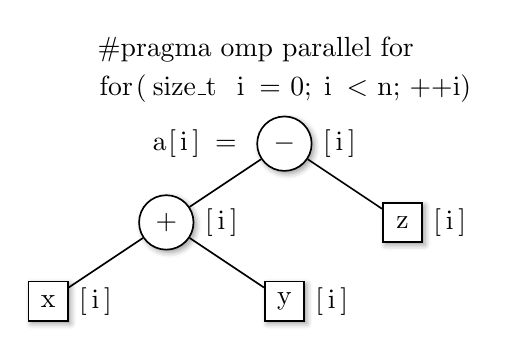
\begin{tikzpicture}
                    \draw (0,0) node(sub)            [treenode,circle]{$-$};
                    \draw (sub) +( 1.50,-1) node(z)  [treenode,minimum size=0.5cm]{z};
                    \draw (sub) +(-1.50,-1) node(add)[treenode,circle]{$+$};
                    \draw (add) +(-1.50,-1) node(x)  [treenode,minimum size=0.5cm]{x};
                    \draw (add) +( 1.50,-1) node(y)  [treenode,minimum size=0.5cm]{y};

                    \draw (sub) -- (add);
                    \draw (sub) -- (z);
                    \draw (add) -- (x);
                    \draw (add) -- (y);

                    \uncover<5->{
                        \draw (sub) +(-2.5, 1.2) node[anchor=west]{\code{#pragma omp parallel for}};
                    }
                    \uncover<2->{
                        \draw (sub) +(-2.5, 0.7) node[anchor=west]{\code{for(size_t i = 0; i < n; ++i)}};
                        \draw (sub) +(-1.8, 0.0) node[anchor=west]{\code{a[i] =}};
                    }
                    \uncover<2> {\draw (sub) +(0.7, 0) node{\code{[i]}};}
                    \uncover<3> {\draw (add) +(0.7, 0) node{\code{[i]}};}
                    \uncover<3->{\draw (z)   +(0.6, 0) node{\code{[i]}};}
                    \uncover<4->{\draw (x)   +(0.6, 0) node{\code{[i]}};}
                    \uncover<4->{\draw (y)   +(0.6, 0) node{\code{[i]}};}
                \end{tikzpicture}
            \end{figure}
        \end{column}
    \end{columns}
\end{frame}

%----------------------------------------------------------------------------
\begin{frame}[fragile]{Source code generation}
    \begin{exampleblock}{Expression:}
        \begin{lstlisting}
a = x + y - z;
        \end{lstlisting}
    \end{exampleblock}
    \begin{exampleblock}{Kernel:}
        \begin{lstlisting}
kernel void vexcl_vector_kernel(
    ulong n,
    global double * prm_1,
    global double * prm_2,
    global double * prm_3,
    global double * prm_4
)
{
    for(size_t idx = get_global_id(0); idx < n; idx += get_global_size(0)) {
        prm_1[idx] = ( ( prm_2[idx] + prm_3[idx] ) - prm_4[idx] );
    }
}
        \end{lstlisting}
    \end{exampleblock}
    \begin{tikzpicture}[overlay,scale=0.8]
        \draw (11,6) node(sub)[treenode,circle]{$-$};
        \draw (sub) +( 1.50,-1) node(z)  [treenode,minimum size=0.5cm]{z};
        \draw (sub) +(-1.50,-1) node(add)[treenode,circle]{$+$};
        \draw (add) +(-1.50,-1) node(x)  [treenode,minimum size=0.5cm]{x};
        \draw (add) +( 1.50,-1) node(y)  [treenode,minimum size=0.5cm]{y};
        \draw (sub) -- (add);
        \draw (sub) -- (z);
        \draw (add) -- (x);
        \draw (add) -- (y);
    \end{tikzpicture}
\end{frame}

%----------------------------------------------------------------------------
\begin{frame}[fragile]{Declaring parameters}
    \begin{exampleblock}{Each terminal knows what parameters it needs:}
        \begin{lstlisting}
/*static*/ void vector::declare_params(std::ostream &src, unsigned &pos)
{
    src << ",\n    global double * prm" << ++pos;
}
        \end{lstlisting}
    \end{exampleblock}
    \vspace{0.5\baselineskip}
    \begin{exampleblock}{An expression just asks its terminals to do the work:}
        \begin{lstlisting}[firstnumber=last]
template <class LHS, class OP, class RHS>
/*static*/ void binary_op<LHS, OP, RHS>::declare_params(std::ostream &src, unsigned &pos)
{
    LHS::declare_params(src, pos);
    RHS::declare_params(src, pos);
}
        \end{lstlisting}
    \end{exampleblock}
\end{frame}

\note{ }

%----------------------------------------------------------------------------
\begin{frame}[fragile]{Building string representation for expression}
    \begin{exampleblock}{}
        \begin{lstlisting}
struct plus {
    static std::string to_string(std::ostream &src) { src << " + "; }
};

/*static*/ void vector::to_string(std::ostream &src, unsigned &pos) {
    src << "prm" << ++pos << "[idx]";
}

template <class LHS, class OP, class RHS>
/*static*/ void binary_op<LHS, OP, RHS>::to_string(std::ostream &src, unsigned &pos) {
    src << "( ";
    LHS::to_string(src, pos);
    OP::to_string(src);
    RHS::to_string(src, pos);
    src << " )";
}
        \end{lstlisting}
    \end{exampleblock}
\end{frame}

\note[itemize]{
\item The obvious observation is that\ldots
}

%----------------------------------------------------------------------------
\begin{frame}[fragile]{Generating kernel source}
    \begin{exampleblock}{}
        \begin{lstlisting}
template <class LHS, class RHS>
std::string kernel_source() {
    std::ostringstream src;

    src << "kernel void vexcl_vector_kernel(\n    ulong n";
    unsigned pos = 0;
    LHS::declare_params(src, pos);
    RHS::declare_params(src, pos);
    src << ")\n{\n"
            "  for(size_t idx = get_global_id(0); idx < n; idx += get_global_size(0)) {\n"
            "    ";
    pos = 0;
    LHS::to_string(src, pos); src << " = ";
    RHS::to_string(src, pos); src << ";\n";
    src << "  }\n}\n";

    return src.str();
}
        \end{lstlisting}
    \end{exampleblock}
\end{frame}

\note{ }

%----------------------------------------------------------------------------
\begin{frame}[fragile]{Generating/launching the kernel on demand}
    \begin{exampleblock}{}
        \begin{lstlisting}
template <class Expr>
const vector& vector::operator=(const Expr &expr) {
    static cl::Kernel krn = build_kernel(device, kernel_source<This, Expr>());

    unsigned pos = 0;

    krn.setArg(pos++, size);       // n
    this->set_args(krn, pos);      // result
    expr.set_args(krn, pos);       // other parameters

    queue.enqueueNDRangeKernel(krn, cl::NullRange, buffer.size(), cl::NullRange);

    return *this;
}
        \end{lstlisting}
    \end{exampleblock}
    \begin{itemize}
        \item The kernel is uniquely identified by the expression type.
            \begin{itemize}
                \item Local static variable may be used to cache the
                    kernel.
                \item The kernel is generated and compiled once, applied many
                    times.
            \end{itemize}
    \end{itemize}
\end{frame}

\note{ }

%----------------------------------------------------------------------------
\begin{frame}{Using Boost.Proto}
    \begin{description}[\quad]
        \item[Problem:] this does not scale very well
            \begin{itemize}
                \item There are unary, binary, n-ary expressions.
                \item There are special terminals requiring either global or
                    local preambles.
                \item There are builtin and user-defined functions.
                \item We need to be able to combine all of the above in an
                    expression.
            \end{itemize}
            \vspace{\baselineskip}
        \item[Solution:] Boost.Proto
            \begin{itemize}
                \item Framework for building Embedded Domain-Specific
                    Languages in \CXX.
                \item Provides tools for constructing, type-checking,
                    transforming and executing expression templates.
            \end{itemize}
    \end{description}
\end{frame}

%----------------------------------------------------------------------------
\begin{frame}[fragile]
    \begin{exampleblock}{Proto grammar}
        \begin{lstlisting}
struct vector_grammar
    : proto::or_<
          proto::and_<
              proto::terminal<proto::_>,
              proto::if_<is_vector_expr_terminal<proto::_value>() >
          >,
          proto::or_<
              proto::unary_plus<vector_grammar>,
              proto::negate<vector_grammar>,
              ...
              proto::plus <vector_grammar, vector_grammar>,
              proto::minus<vector_grammar, vector_grammar>,
              ...
          >,
          ...
      >
{};
        \end{lstlisting}
    \end{exampleblock}
    \begin{tikzpicture}[remember picture,overlay]
        \node[anchor=north east,yshift=-2cm] at (current page.north east) {
            
\includegraphics[width=3.6cm]{owl1}
        };
    \end{tikzpicture}
\end{frame}

%----------------------------------------------------------------------------
\begin{frame}[fragile]
    \begin{exampleblock}{Proto contexts}
        \begin{adjustbox}{width=0.9\textwidth, height=\textheight, keepaspectratio}
            \begin{minipage}{\textwidth}
                \begin{lstlisting}
template <class Term> struct partial_vector_expr {
    static void get(std::ostream &os, unsigned &pos) { os << "prm_" << ++pos; }
};
struct vector_expr_context {
    std::ostream &os; unsigned pos = 0;
    template <typename Expr, typename Tag = typename Expr::proto_tag> struct eval;

    template <typename Expr> struct eval<Expr, boost::proto::tag::plus> {
        typedef void result_type;
        void operator()(const Expr &expr, vector_expr_context &ctx) const {
            os << "( ";     proto::eval(proto::left (expr), ctx);
            os << " + ";    proto::eval(proto::right(expr), ctx); os << " )";
        }
    };
    ...
    template <typename Expr> struct eval<Expr, boost::proto::tag::terminal> {
        typedef void result_type;
        void operator()(const Expr &expr, vector_expr_context &ctx) const {
            partial_vector_expr<typename proto::result_of::value<Expr>::type>::get(os, ctx.pos);
        }
    };
};
                \end{lstlisting}
            \end{minipage}
        \end{adjustbox}
    \end{exampleblock}
    \begin{onlyenv}<1>
        \begin{tikzpicture}[remember picture,overlay]
            \node[anchor=north east,yshift=-2cm] at (current page.north east) {
                
\includegraphics[width=3.6cm]{owl2}
            };
        \end{tikzpicture}
    \end{onlyenv}
    \begin{onlyenv}<2>
        \begin{tikzpicture}[remember picture,overlay]
            \node[anchor=north east,yshift=-2cm] at (current page.north east) {
                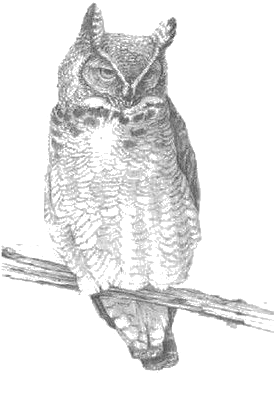
\includegraphics[width=3.6cm]{owl3}
            };
        \end{tikzpicture}
    \end{onlyenv}
\end{frame}

%----------------------------------------------------------------------------
\begin{frame}[fragile]{Adding new terminals}
    \begin{itemize}
        \item Once the DSL engine is done, adding new terminals is easy:
    \end{itemize}
    \begin{exampleblock}{}
        \begin{lstlisting}[escapechar=@]
x = sin( 2 * M_PI * @{\bf vex::element\_index()}@ / n );
        \end{lstlisting}
    \end{exampleblock}
    \begin{exampleblock}{Let Proto know the terminal is allowed in vector
        expressions:}
        \begin{lstlisting}
struct elem_index {
    size_t offset;
    size_t length;
};

template <> struct is_vector_expr_terminal< elem_index > : std::true_type {};

inline auto element_index(size_t offset = 0, size_t length = 0) {
    return proto::as_expr<vector_domain>( elem_index{offset, length} );
}
        \end{lstlisting}
    \end{exampleblock}
\end{frame}

\note{ }

%----------------------------------------------------------------------------
\begin{frame}[fragile]
    \begin{exampleblock}{Parameter declaration:}
        \begin{lstlisting}
template <> struct kernel_param_declaration<elem_index> {
    static std::string get(
        const elem_index&, const cl::Device&, const std::string &prm_name)
    {
        return ",\n\t" + type_name<size_t>() + " " + prm_name;
    }
};
        \end{lstlisting}
    \end{exampleblock}
    \vspace{0.5\baselineskip}
    \begin{exampleblock}{Contribution to expression string:}
            \begin{lstlisting}
template <> struct partial_vector_expr<elem_index> {
    static std::string get(
            const elem_index&, const cl::Device&, const std::string &prm_name)
    {
        return "(" + prm_name + " + idx)";
    }
};
            \end{lstlisting}
    \end{exampleblock}
\end{frame}

\note{ }

%----------------------------------------------------------------------------
\begin{frame}[fragile]
    \begin{exampleblock}{Setting kernel arguments:}
        \begin{lstlisting}
template <> struct kernel_arg_setter<elem_index> {
    static void set(
        const elem_index &term, cl::Kernel &krn, unsigned /* device */,
        size_t index_offset, unsigned &position)
    {
        krn.setArg(position++, term.offset + index_offset);
    }
};
        \end{lstlisting}
    \end{exampleblock}
    \vspace{\baselineskip}
    \begin{itemize}
        \item Done! We can use \code{vex::element_index()} in arbitrary
            vector expressions.
    \end{itemize}
\end{frame}

\note{}

\section{Backends}

%----------------------------------------------------------------------------
\begin{frame}{Supporting different backends}
    \begin{itemize}
        \item Supported backends:
            \begin{itemize}
                \item OpenCL (Khronos \CXX bindings)
                \item OpenCL (Boost.Compute)
                \item NVIDIA CUDA
            \end{itemize}
            \vspace{\baselineskip}

        \item Differences between backends:
            \begin{itemize}
                \item Host-side API
                \item Compute kernel language
                \item JIT compilation support
            \end{itemize}
    \end{itemize}
\end{frame}

%----------------------------------------------------------------------------
\begin{frame}[fragile]{Abstraction layer}
    \begin{itemize}
        \item Any backend in VexCL consists of:
            \vspace{0.5\baselineskip}

            \begin{tabular}{ll}
                \verb|filter.hpp|        & Device filters            \\
                \verb|device_vector.hpp| & Memory abstraction        \\
                \verb|source.hpp|        & Source generation         \\
                \verb|compiler.hpp|      & Compiling compute kernels \\
                \verb|kernel.hpp|        & Compute kernel            \\
                \verb|context.hpp|       & Host-side objects         \\
            \end{tabular}
    \end{itemize}
\end{frame}

%----------------------------------------------------------------------------
\begin{frame}[fragile]{Source generation}
    \begin{exampleblock}{}
        \begin{lstlisting}
class source_generator {
    source_generator &kernel(const std::string &name);

    template <typename Return>
    source_generator& function(const std::string &name);

    template <typename Param>
    source_generator& parameter(const std::string &name);

    source_generator& open(const std::string &bracket);
    source_generator& close(const std::string &bracket);

    source_generator& new_line();
    source_generator& grid_stride_loop(
                const std::string &idx = "idx", const std::string &bnd = "n");

    template <class T>
    friend source_generator& operator<<(source_generator &src, const T &t);
};
        \end{lstlisting}
    \end{exampleblock}
\end{frame}

%----------------------------------------------------------------------------
\begin{frame}[fragile]{Source generation: example}
    \begin{columns}
        \begin{column}{0.45\textwidth}
            \begin{exampleblock}{}
                \begin{lstlisting}
source_generator src;
src.function<double>("squared_radius")
    .open("(")
    .parameter<double>("a")
    .parameter<double>("b")
    .close(")").open("{");
src.new_line() << "return a*a + b*b;";
src.close("}");
std::cout << src.str() << std::endl;
                \end{lstlisting}
            \end{exampleblock}
        \end{column}
        \begin{column}{0.45\textwidth}
            \begin{exampleblock}{}
                \vspace{0.5\baselineskip}
                \begin{lstlisting}
double squared_radius
(
  double a,
  double b
)
{
  return a*a + b*b;
}
                \end{lstlisting}
                \vspace{0.5\baselineskip}
            \end{exampleblock}
        \end{column}
    \end{columns}
\end{frame}

\section{Generic code}

%----------------------------------------------------------------------------
\begin{frame}{Writing generic code}
\end{frame}

\section{Limitations of ET}

%----------------------------------------------------------------------------
\begin{frame}[fragile]{Limitations of expressions templates}
    \begin{exampleblock}{Impossible to alter execution details for an expression:}
        \begin{lstlisting}
vex::vector<double> x({q1}, n);
vex::vector<double> y({q2}, n);
x = 2 * y;
        \end{lstlisting}
    \end{exampleblock}
    \begin{itemize}
        \item Which queue to use?
        \item How to configure the kernel?
    \end{itemize}

    \vspace{\baselineskip}

    \begin{exampleblock}{One-by-one execution may be ineffective:}
        \begin{lstlisting}
u = x + y;
v = x - y;
        \end{lstlisting}
    \end{exampleblock}
    \begin{itemize}
        \item \code{x} and {y} are read twice.
        \item How to fuse the expressions into a single kernel?
    \end{itemize}
\end{frame}

\note{}

\end{document}
